\climbingarea{South Freeport Coffin Area}{%
    \climbheader{This is in Freeport..}{This is public access Land Trust land.}{Park at the Pine St/South Freeport Roard intersection pullout and walk back up Pine St 200 ft.}{The area is often wet, but The Coffin boulder stays dry.}
    \climbingarea{The Coffin Boulder}{The Coffin Boulder is pretty cool.}{%
        % A minipage is basically a small box of content that we will use to encapsulate our image. We will make it as wide as a line of text. This is used to maintain the formatting of the other text on the page.
        \begin{minipage}{\linewidth}%
          % We want to center the image within the minipage.
          \centering
          % This particular file is likely marked as "rotated" in the EXIF data, which LaTeX ignores...so we have to manually roate it here with the "angle" setting.
          % If you want the image smaller, you can change the width to '.5\linewidth' or some other value like that.
          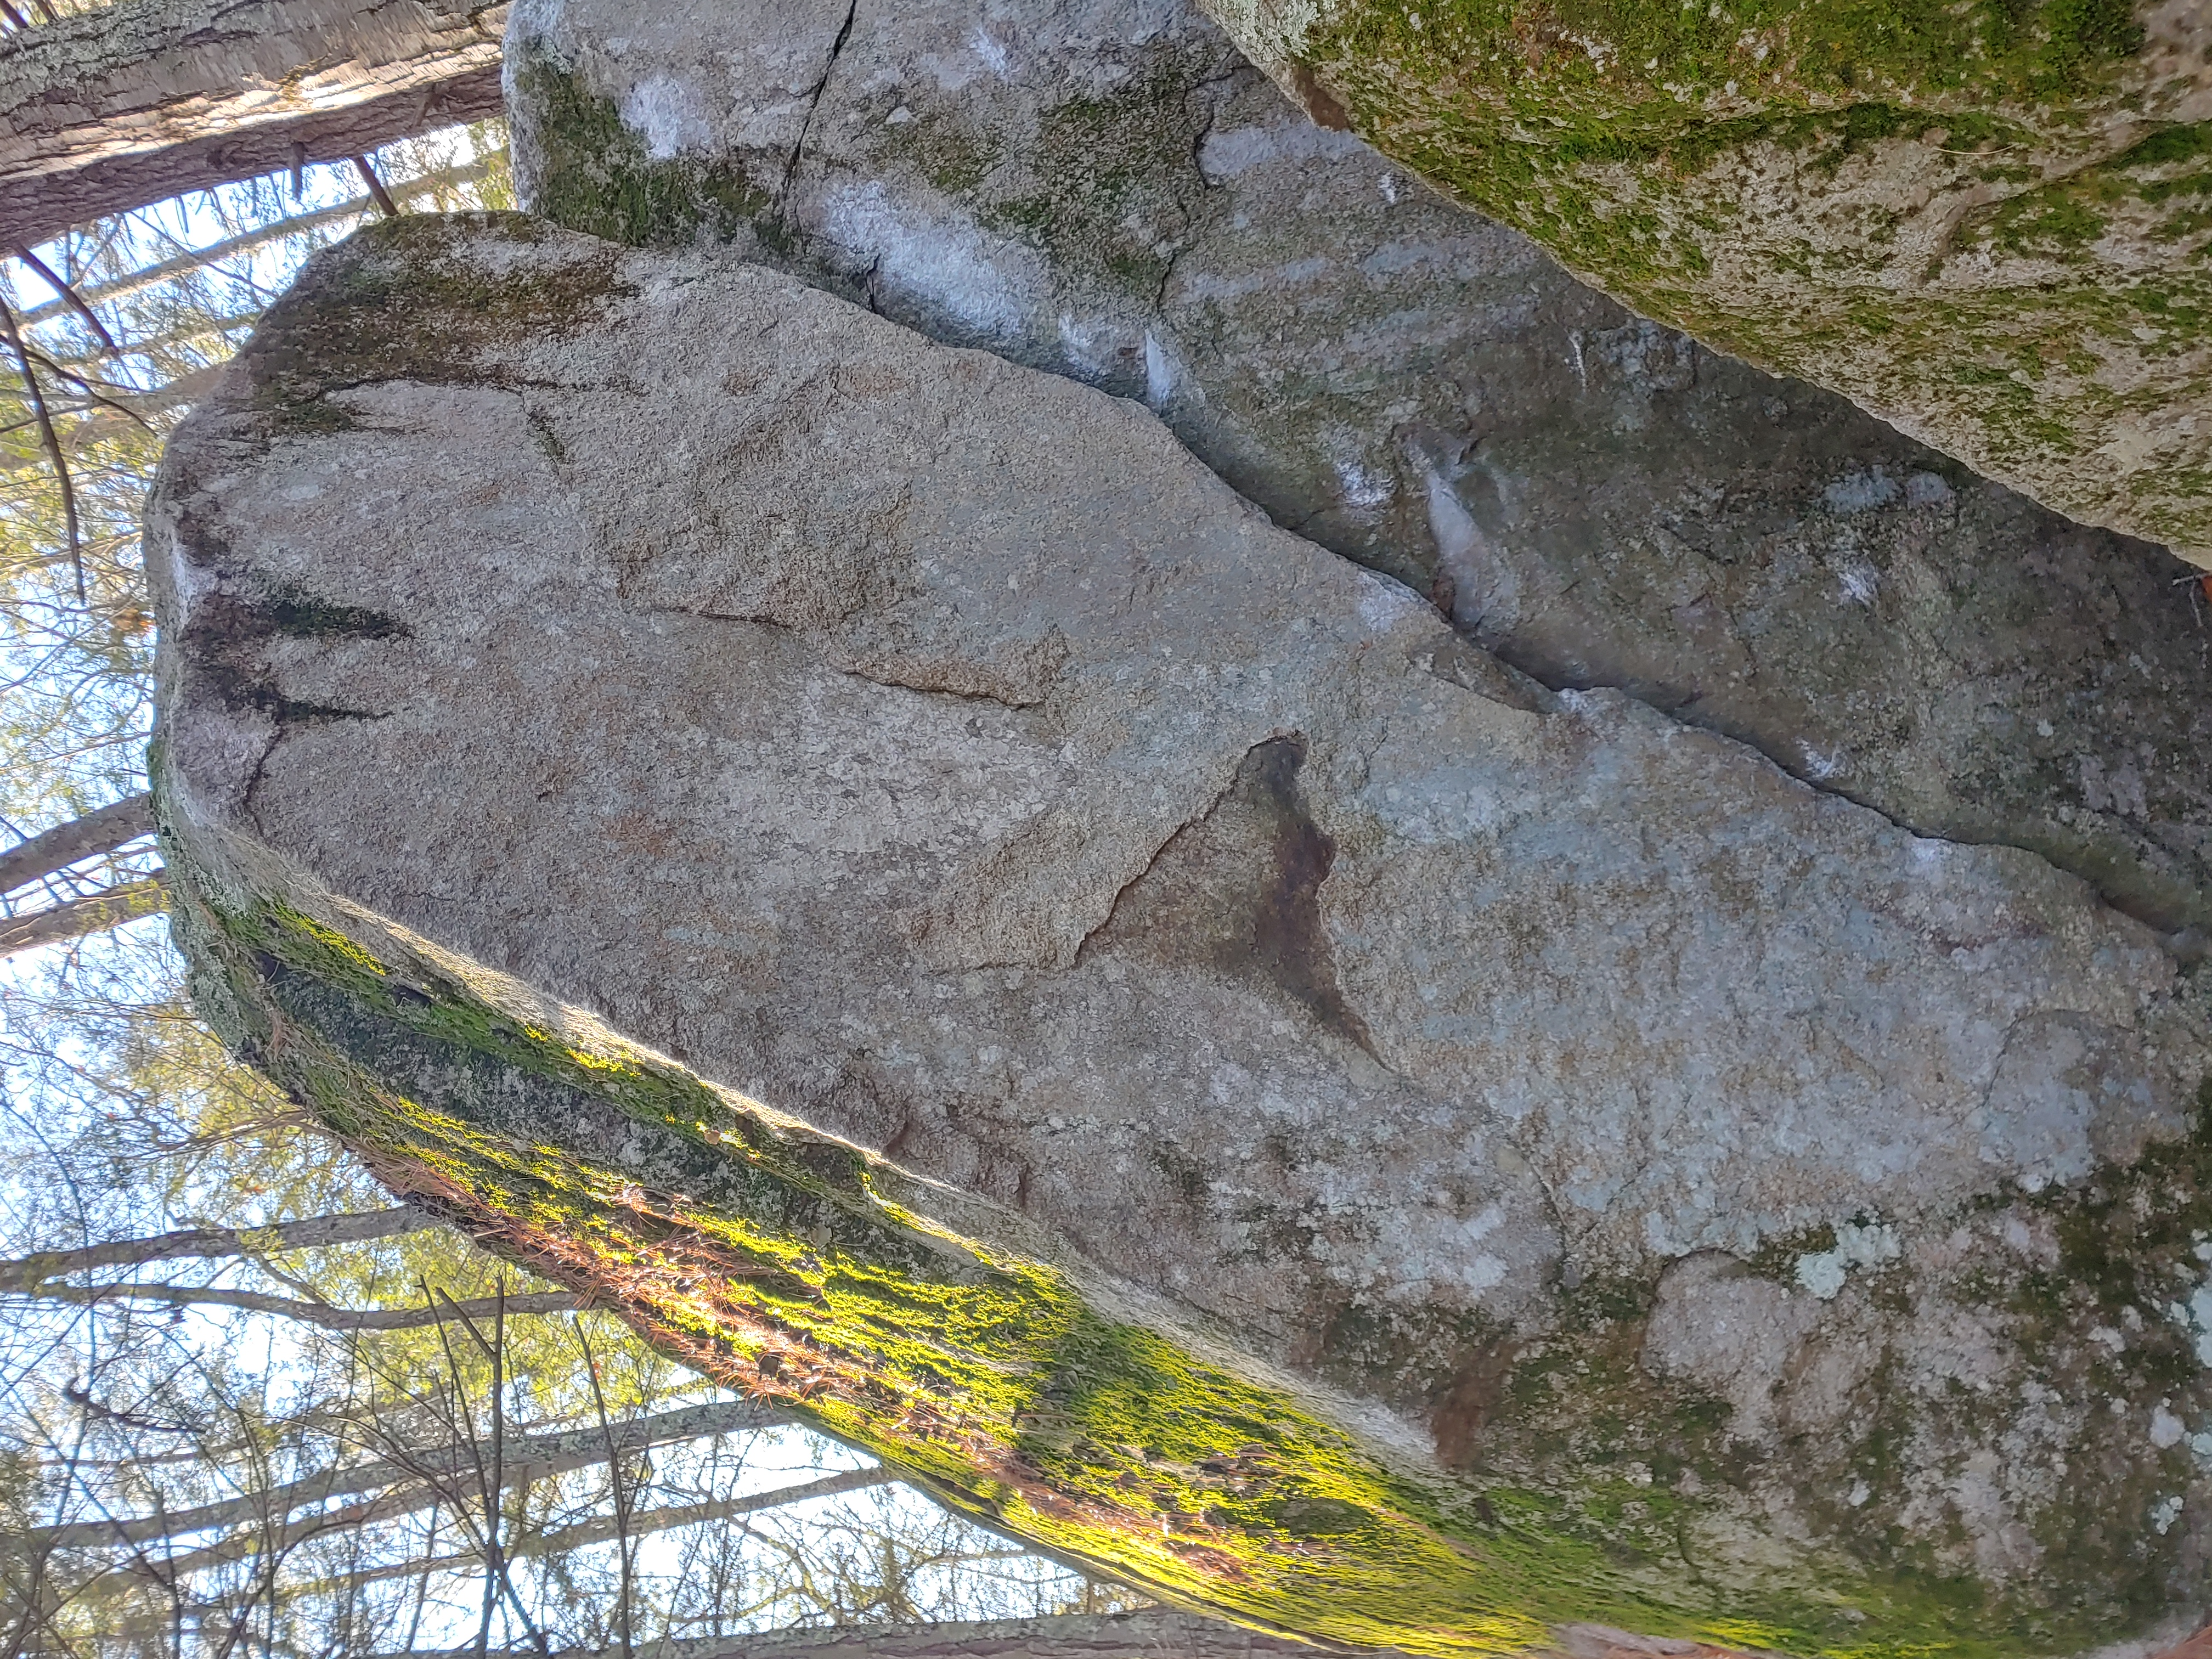
\includegraphics[angle=270,width=.8\linewidth]{1201251115_HDR.jpg}
          \captionof{figure}{The Coffin V8/9}
        \end{minipage}
        % This is a comment
        % the syntax of \boulderproblem is:
        % \boulderproblem[number of stars]{Name}{Grade}{Description}{Height}{FA}
        \boulderproblem[4]{The Coffin}{V8/9}{Sit-start with hands on either arete with thumbcatch. Climb up the prow with compression, topping out to the left..}{10}{Ben Yunker?}
        \boulderproblem[4]{Podule}{V6}{Sit-start with hands on the right side of sloper cracks. Climb up and left on rough slopers.}{10}{unknown}
    }
}{}

\climbingarea{Ocean Point}{%
    \climbheader{This is in Boothbay}{There is a neat shoreline walk here, and at the very end are some boulders.}{Park at the public parking along Shore Road or the dedicated Ocean Point Trust parking lot.}
    \climbingarea{The Bends Boulder}{About a half mile from parking, look back the way you came and you'll see this beauty.}{%
        % A minipage is basically a small box of content that we will use to encapsulate our image. We will make it as wide as a line of text. This is used to maintain the formatting of the other text on the page.
        \begin{minipage}{\linewidth}%
          % We want to center the image within the minipage.
          \centering
          % This particular file is likely marked as "rotated" in the EXIF data, which LaTeX ignores...so we have to manually roate it here with the "angle" setting.
          % If you want the image smaller, you can change the width to '.5\linewidth' or some other value like that.
          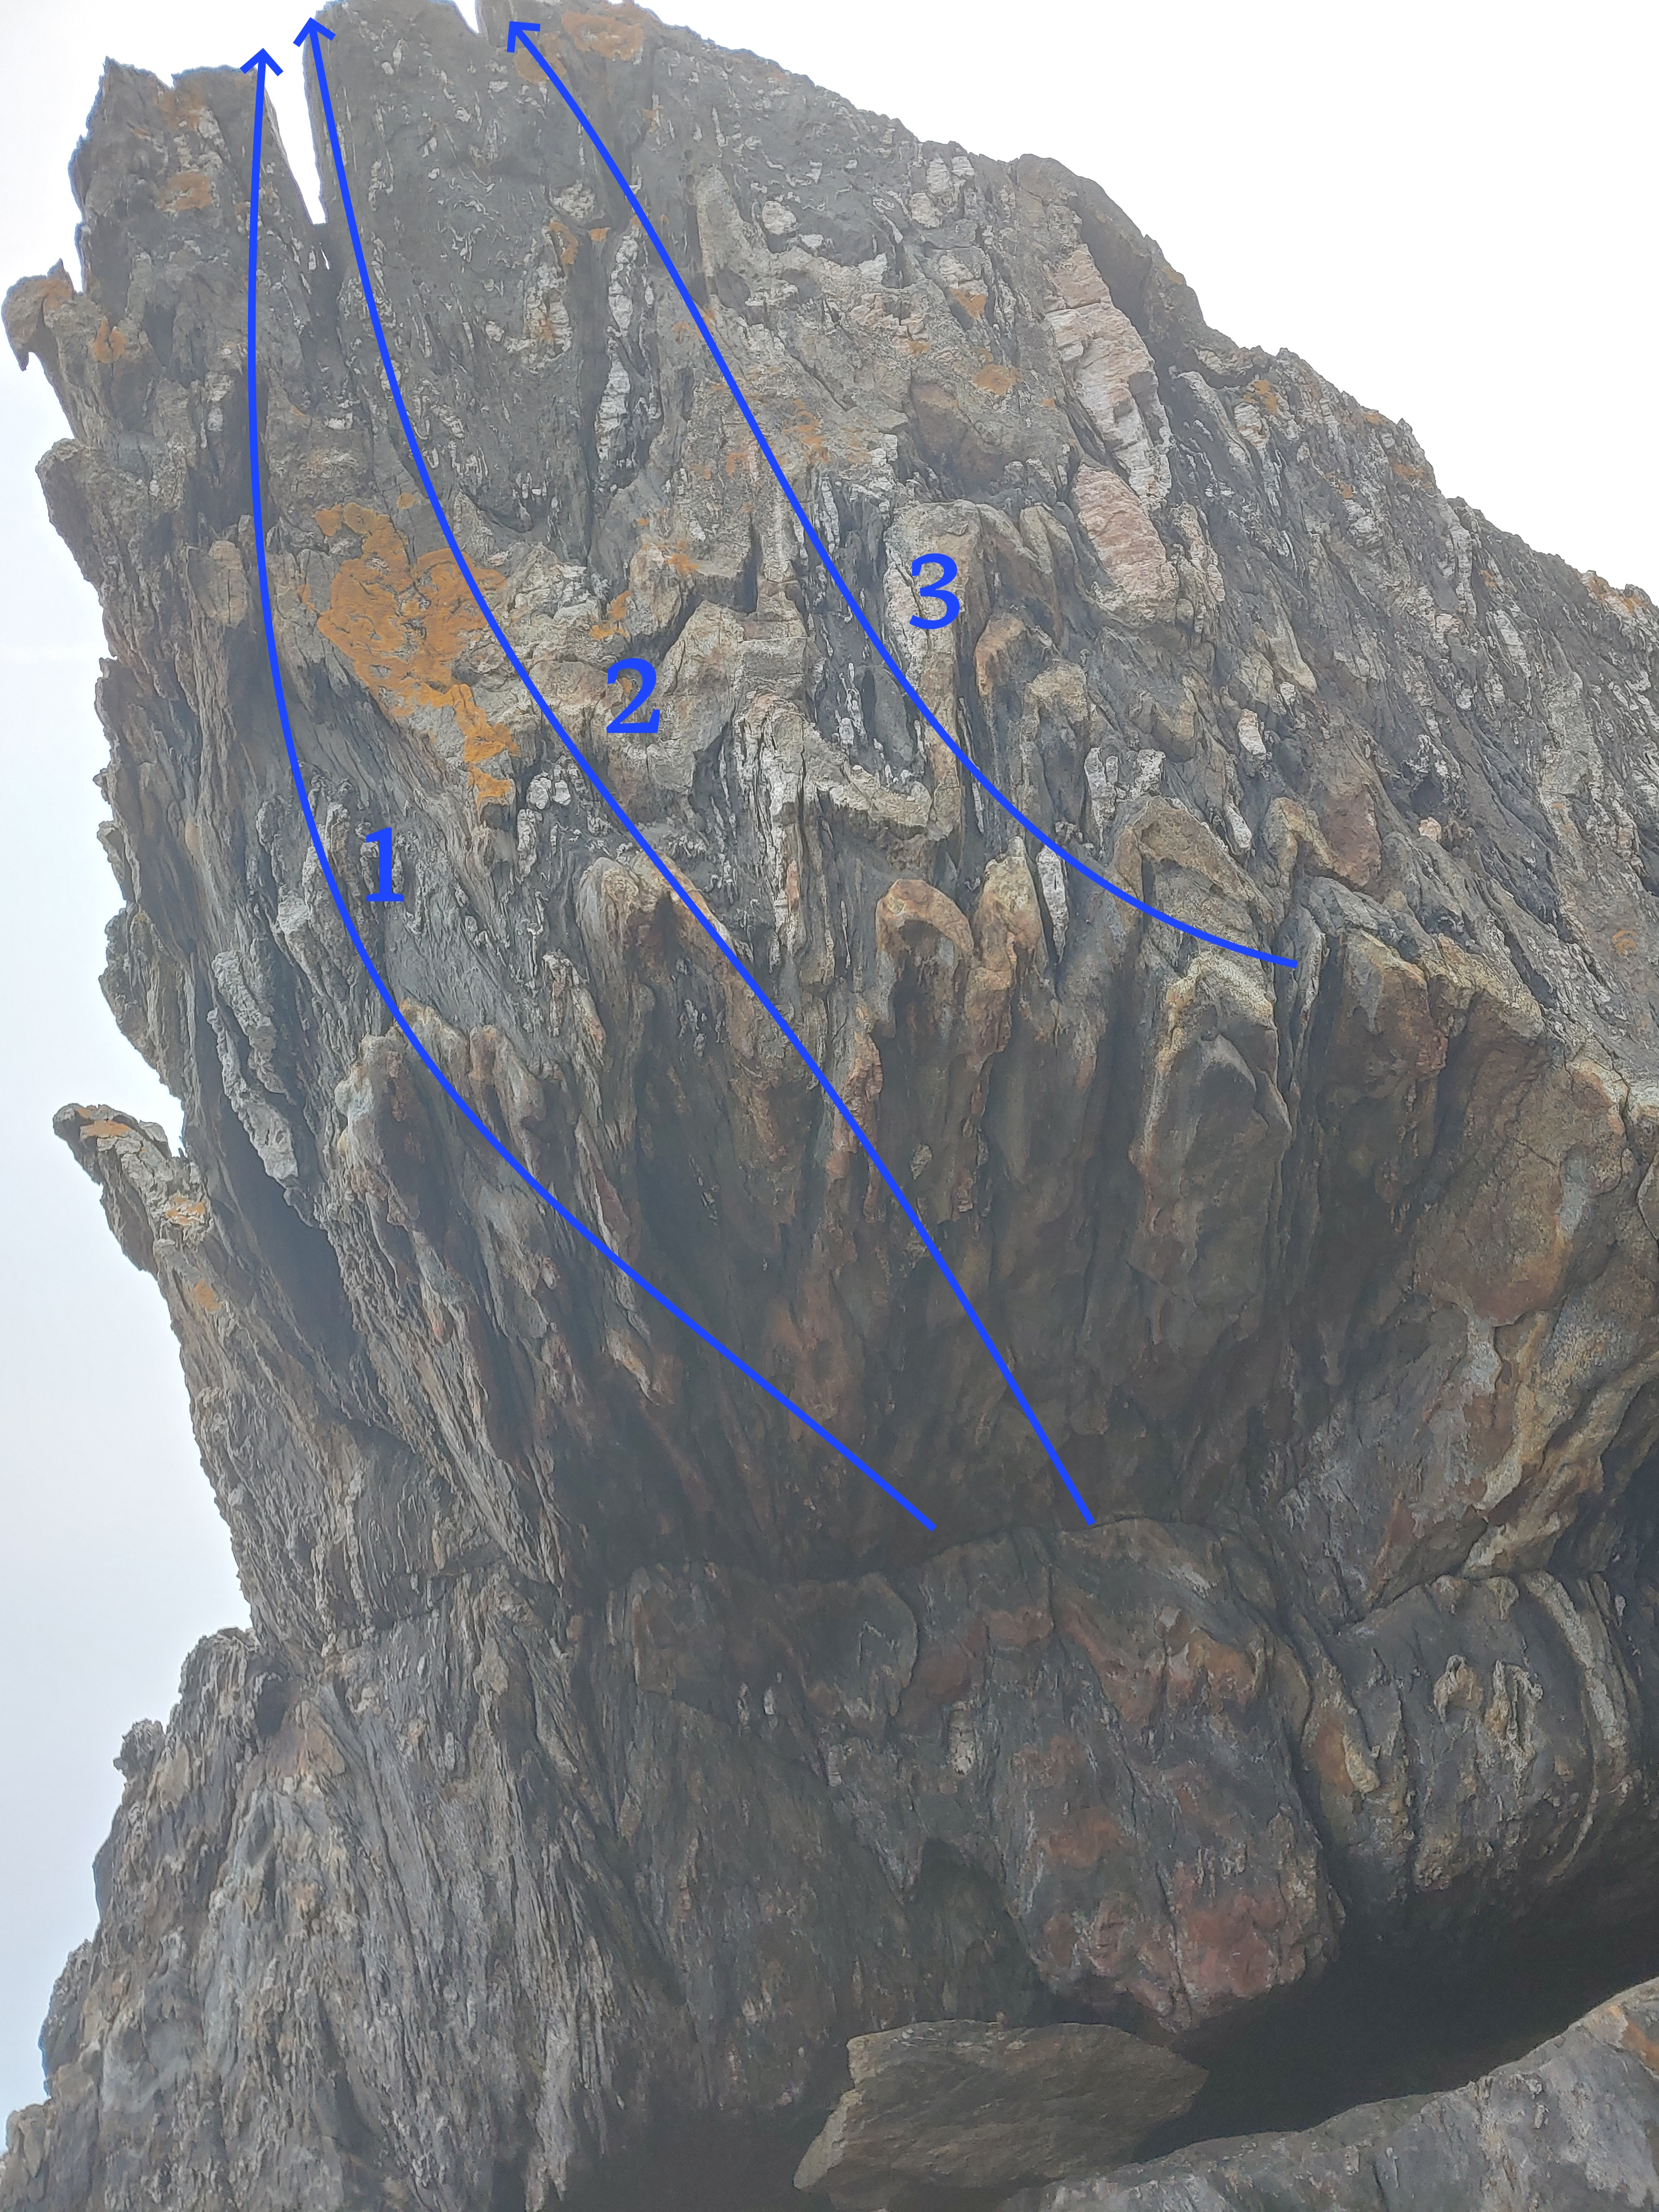
\includegraphics[width=.8\linewidth]{bends.jpg}
          \captionof{figure 2}{The Bends Boulder}
        \end{minipage}
        % This is a comment
        % the syntax of \boulderproblem is:
        % \boulderproblem[number of stars]{Name}{Grade}{Description}{Height}{FA}
        \boulderproblem[3]{Sugar Kelp Welp}{V2}{Start in the back of cave. Big move up to juggy undercling rail on roof then another big move out to face. Top out left, straight up, or right, all on jugs.}{12}{unknown}
        \boulderproblem[4]{The Bends}{V5}{Start on juggy slot at back of the cave and climb straight out roof using some combination of slots, pinches, and gastons to work into a position to reach one of the jugs at the base of the headwall. Jug up to the very good lip.}{12}{Toby fka}
        \boulderproblem[4]{Racing Marlin}{V1}{Campus/hanging start on the right face on jugs at base of headwall. Find more jugs as you go straight up to the good lip.}{12}{unknown}
    }} {}

\climbingarea{Nesting Test}{%
    \climbheader{This is a spot with multiple sub-areas}{Cool spot overall.}
    \climbingarea{Area 1}{Boulder Natural}{%
        \climbingarea{Sub-Area 1}{A nested area}{%
            \boulderproblem[3]{Birds in the Nest}{V2}{Start halfway and go right.}{12}{unknown}
        }
        \climbingarea{Sub-Area 2}{Another nested area}{%
            \boulderproblem[3]{Babies in the Nest}{V2}{Start low, go high.}{12}{unknown}
        }
    }
}

